\chapter{Second Weight Estimation}

\section{Weight Estimate}
\begin{table}[h!]
 \begin{center}
 \begin{tabular}{|c| c |c |c|} 
 \hline
 Components & Weight(grams) & Quantity & Total Weight(grams) \\ [0.5ex] 
 \hline
 Propeller & 7.5 & 4 & 7.5*4=30 \\ 
 \hline
 Motor & 23 & 4 & 23*4=92 \\
 \hline
 Flight Control Board & 60  & 1 & 60*1=60 \\
 \hline
 Electronic speed controller & 100 & 4 & 100*4=400 \\ 
 \hline
 Base weight & 200 & 1 & 200*1 = 200 \\ 
 \hline
 Camera weight & 120 & 1 & 100*1=100 \\ 
 \hline
 Battery & 160 & 1 & 160*1=160 \\ 
 \hline
 Bolts & 20 & - & 20 \\ 
 \hline
 Locking nuts & 20 & - & 20 \\ 
 \hline
 Wires & 30 & - & 30 \\ 
 \hline
\end{tabular}
\caption{\label{table:weight_estimation}Second Weight Estimation}
\end{center}

\end{table}
Total weight = 30+92+60+400+200+100+160+20+20+30 = 1112 grams
\section{Thrust Calculation}

\subsection{Sample Calculation}

The analytical calculations need to be done initially to verify whether the data obtained is feasible or not.We have done a sample calculation by considering an 
approximate weight of 1000 grams.Let us consider a thrust to weight ratio of 2 as is the general trend while designing drones.Head space is taken as 20 \% and hence the thrust to weight ratio finally changes to 2.4

Therefore, the net thrust that the motors need to provide is 1000 * 2.4 = 2400 grams.The thrust required per motor and thereof for one propeller is 2400/4 = 600 grams.
For different size of propeller, with different rpm values we can achieve above thrust.

Let us consider the propeller size to be 8*4 and motor rpm around 10500,which is generally used with quadcopters of the frame that we have thought of.Here 8 is the diameter in inches and 4 is the pitch.Pitch is defined as the linear movement it will travel in 1 second.The thrust obtained is 605 grams if we are using the above propeller with the mentioned motor speed, from the formula that is given in Figure 2.1.For obtaining 10500 rpm the KV rating which is given by rpm per volt is 2570.Now in most quadcopters we are using a 3cell 11.1V Lithium Polymer battery.Therefore the net rpm of motion is 28527 rpm

If propeller diameter is 10 inchess then motor rpm becomes 1/3rd that is 9509 rpm.
Similarly, when 5 inch diameter is chosen the rpm is reduced by 50 \%, that is it becomes 14263.5 rpm which is more than required.

Therefore, a propeller of size 8*4 is analytically feasible to be used to get a net thrust of approximately 1000 grams.

The battery weight for the given configuration is 160 grams and the motor weight is 23*4 = 92 grams.The net weight of 4 propellers is 30 grams.Now, considering the weight that we have obtained which is 1112 grams.The required thrust per propeller will be (1112*2.4)/4 which is 670 grams.The corresponding rpm is 11000 rpm.
Hence, 8*4 propeller with selected motor and battery can give us required rpm and the thrust needed.



\begin{itemize}

\item The analytical calculations are as follows:

\item Estimated Weight of drone = 1112 grams

\item Thrust/Weight = 2

\item Headspace given for thrust = 20 \%

\item Net thrust required = 2.4 * 1112 grams = 2669 grams

\item Net thrust required per motor = 670 grams

\item Specification of propeller:
\begin{enumerate}
\item Diameter = 8 inches
\item pitch = 4 inches
\end{enumerate}
\end{itemize}

\subsection{Motor Specification}
\itemize

\item Motor: Avionic M2226/18 KV2570 MICRO brushless motor

\item KV (rpm/v): 2570

\item Power: 80W

\item Winds: 18

\item Resistance: 327 mOhm

\item Idle current: 0.8 A

\item Weight: 23 gms



\subsection{Formula used for thrust calculation}

\begin{figure}[H]
	\centering
	
	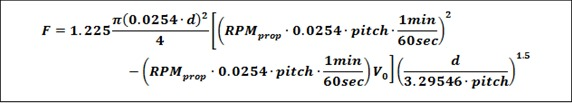
\includegraphics[scale=0.8]{thrustformula.jpeg}
	
	\label{fig:boat}
\end{figure}




\begin{figure}[H]
\centering

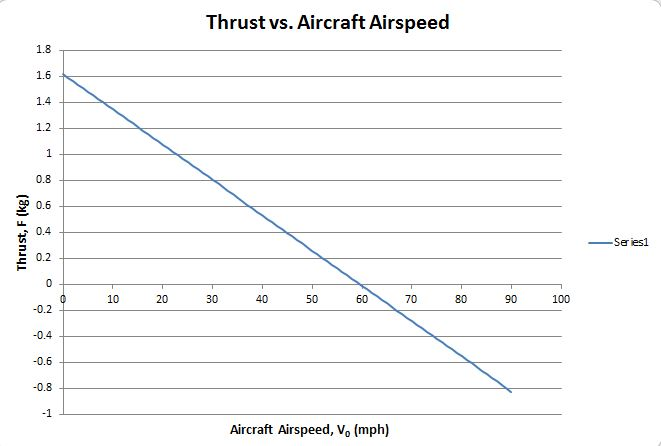
\includegraphics[scale=0.8]{ThrustGraph.jpeg}
\label{fig:boat}
\caption{\label{fig:Thrust_v/s_speed}Thrust v/s Speed}
.\end{figure}




\subsection{Battery Specification}

\item Minimum Capacity: 2200mAh

\item Configuration: 3S1P / 11.1v / 3Cell

\item Constant Discharge: 25C

\item Peak Discharge (10sec): 35C
\section{Procedure}

\item Decide appropriate dimension of propeller.
\item Choose suitable RPM of motor.
\item Get the required static thrust from the table.
\item Iterate the dimensions until you get the required thrust which is 672 g of thrust.
\item After fixing the dimension and RPM of motor, find suitable LiPo battery
\item RPM = KV * Battery voltage
RPM = 2570 * 11.1 = 28500
\item This is the RPM of motor without propeller.After using propeller RPM reduces by 2.5 times approximately.
\item Net RPM = 11410 (estimated)
\item After finalizing the battery, fix the Electronic speed controller.

  
\section{Conclusion} 
The weight of the inflatable drone is estimated to be around 1112gm.The estimated static thrust produced is 6.636 N.In the next phase, after performing successive iterations we will finalize the weight of the drone and perform dynamic thrust calculations.

